\documentclass[aspectratio=169,10pt]{beamer}

\usepackage{amsmath,amssymb}
\usepackage{booktabs}
\usepackage{array}
\usepackage{tikz}
\usepackage{hyperref}
\usetikzlibrary{arrows.meta,positioning,shapes.geometric,calc}

\usetheme{default}

% ---------------------------------------------------------
% COLORS
% ---------------------------------------------------------
\definecolor{Navy}{RGB}{25,43,70}
\definecolor{Blue}{RGB}{48,93,150}
\definecolor{Teal}{RGB}{35,130,135}
\definecolor{LightBlue}{RGB}{237,244,251}
\definecolor{LightTeal}{RGB}{233,247,246}
\definecolor{LightOrange}{RGB}{253,244,231}
\definecolor{LightPurple}{RGB}{244,241,250}
\definecolor{DarkGray}{RGB}{60,65,70}
\definecolor{MediumGray}{RGB}{105,110,115}
\definecolor{LightGray}{RGB}{246,247,249}

% ---------------------------------------------------------
% BEAMER STYLE
% ---------------------------------------------------------
\setbeamertemplate{navigation symbols}{}
\setbeamersize{text margin left=0.55cm,text margin right=0.55cm}

\setbeamercolor{normal text}{fg=DarkGray,bg=white}
\setbeamercolor{structure}{fg=Blue}
\setbeamercolor{frametitle}{fg=white,bg=Navy}
\setbeamerfont{frametitle}{size=\large,series=\bfseries}

\setbeamertemplate{frametitle}{%
  \nointerlineskip%
  \begin{beamercolorbox}[wd=\paperwidth,ht=0.78cm,dp=0.14cm,leftskip=0.55cm]{frametitle}%
    \usebeamerfont{frametitle}\insertframetitle%
  \end{beamercolorbox}%
}

\setbeamertemplate{footline}{%
  \leavevmode%
  \hbox{%
    \begin{beamercolorbox}[wd=.78\paperwidth,ht=0.25cm,dp=0.06cm,leftskip=0.55cm]{author in head/foot}%
      \color{MediumGray}\tiny Retail Promotion Planning and Campaign Optimization%
    \end{beamercolorbox}%
    \begin{beamercolorbox}[wd=.22\paperwidth,ht=0.25cm,dp=0.06cm,rightskip=0.55cm]{author in head/foot}%
      \color{MediumGray}\tiny\hfill\insertframenumber/12%
    \end{beamercolorbox}%
  }%
}

\setbeamertemplate{blocks}[rounded][shadow=false]
\setbeamercolor{block title}{fg=Navy,bg=LightBlue}
\setbeamercolor{block body}{fg=DarkGray,bg=LightBlue!45}

\setbeamertemplate{itemize item}{\color{Teal}\scriptsize$\bullet$}
\setbeamertemplate{itemize subitem}{\color{Teal}\scriptsize$\bullet$}

% ---------------------------------------------------------
% TIKZ STYLES
% ---------------------------------------------------------
\tikzset{
  flow/.style={
    rectangle, rounded corners=3pt,
    minimum width=2.30cm, minimum height=0.70cm,
    text width=2.30cm, align=center,
    draw=Navy, line width=0.7pt,
    fill=LightBlue, font=\scriptsize
  },
  flowteal/.style={
    rectangle, rounded corners=3pt,
    minimum width=2.30cm, minimum height=0.70cm,
    text width=2.30cm, align=center,
    draw=Teal, line width=0.7pt,
    fill=LightTeal, font=\scriptsize
  },
  floworange/.style={
    rectangle, rounded corners=3pt,
    minimum width=2.30cm, minimum height=0.70cm,
    text width=2.30cm, align=center,
    draw=Blue, line width=0.7pt,
    fill=LightOrange, font=\scriptsize
  },
  flowpurple/.style={
    rectangle, rounded corners=3pt,
    minimum width=2.30cm, minimum height=0.70cm,
    text width=2.30cm, align=center,
    draw=Navy, line width=0.7pt,
    fill=LightPurple, font=\scriptsize
  },
  model/.style={
    rectangle, rounded corners=5pt,
    minimum width=3.7cm, minimum height=1.25cm,
    text width=3.7cm, align=center,
    draw=Blue, line width=0.8pt,
    fill=LightOrange, font=\scriptsize
  },
  modelteal/.style={
    rectangle, rounded corners=5pt,
    minimum width=3.7cm, minimum height=1.25cm,
    text width=3.7cm, align=center,
    draw=Teal, line width=0.8pt,
    fill=LightTeal, font=\scriptsize
  },
  outputbox/.style={
    rectangle, rounded corners=5pt,
    minimum width=3.7cm, minimum height=0.70cm,
    text width=3.7cm, align=center,
    draw=Navy, line width=0.8pt,
    fill=LightPurple, font=\scriptsize
  },
  arr/.style={-{Stealth[length=2mm]}, line width=0.8pt, draw=DarkGray}
}

% ---------------------------------------------------------
% TITLE
% ---------------------------------------------------------
\title{Retail Promotion Planning and Campaign Optimization}
\subtitle{An Operations Research Decision-Support System}
\author{Group Members}
\institute{Amrita School of Artificial Intelligence\\Amrita Vishwa Vidyapeetham, Coimbatore}
\date{August 2026}

\begin{document}

% =========================================================
% 1 TITLE
% =========================================================
\begin{frame}[plain]

\vspace{0.65cm}

\begin{columns}[c]

% =========================================================
% Vertical accent line
% =========================================================
\begin{column}{0.06\textwidth}

\begin{tikzpicture}
\fill[Teal] (0,0) rectangle (0.16,5.0);
\end{tikzpicture}
\end{column}

% =========================================================
% Main content
% =========================================================
\begin{column}{0.88\textwidth}

% Title
{\fontsize{26}{31}\selectfont
\color{Navy}
\textbf{Retail Promotion Planning}}\\[-1mm]

{\fontsize{26}{31}\selectfont
\color{Navy}
\textbf{and Campaign Optimization}}

\vspace{0.55cm}

% Group number
{\large
\textbf{Group Number:} \color{Teal}\textbf{D13}
}

\vspace{0.35cm}

% Group members heading
{\large
\color{Navy}
\textbf{Group Members:}
}

\vspace{0.18cm}

% Members
{\normalsize
\textbf{Vishnu} -- CB.SC.U4AIE23352\\[2.5mm]
\textbf{Siva Charan} -- CB.SC.U4AIE23305\\[2.5mm]
\textbf{Srikar} -- CB.SC.U4AIE23355
}

\end{column}

\end{columns}

\end{frame}
% =========================================================
% 2 INTRODUCTION
% =========================================================
\begin{frame}{Introduction}

\vspace{0.35cm}

\begin{itemize}

    \item Retailers generate large volumes of transaction, promotion,
    campaign, and customer-level data.

    \vspace{0.35cm}

    \item Historical retail data can provide valuable insights into
    product performance, promotional effects, and customer behavior.

    \vspace{0.35cm}

    \item Retail planning decisions are constrained by limited
    promotional resources and targeted marketing capacity.

    \vspace{0.35cm}

    \item Operations Research can transform these insights into
    optimal, constraint-aware decisions for retail planning.

\end{itemize}

\end{frame}

% =========================================================
% 3 PROBLEM
% =========================================================
% =========================================================
% 3. PROBLEM STATEMENT
% =========================================================
\begin{frame}{Problem Statement}

\vspace{0.35cm}

\begin{itemize}

    \item Retail promotion and campaign planning involve complex
    decisions that must balance business value with limited resources.

    \vspace{0.3cm}

    \item Historical retail data provides information about
    product promotions, customer purchases, campaign responses,
    and demographic characteristics.

    \vspace{0.3cm}

    \item Simple ranking-based approaches may ignore operational
    constraints such as limited display, mailer, and campaign capacity.

    \vspace{0.3cm}

    \item Campaign targeting must also consider strategic demographic
    goals that may conflict with purely value-based customer selection.

    \vspace{0.3cm}

    \item An Operations Research framework is therefore required to
    determine optimal promotion and targeting decisions under these constraints.

\end{itemize}

\end{frame}

% =========================================================
% 4 OBJECTIVES
% =========================================================
% =========================================================
% 4. OBJECTIVES
% =========================================================
\begin{frame}{Objectives}

\vspace{0.35cm}

\begin{itemize}

    \item To preprocess and analyze historical retail data to
    derive reliable parameters for the proposed optimization models.

    \vspace{0.3cm}

    \item To optimize the allocation of Display, Mailer, or Both
    promotions across products under limited promotional resources.

    \vspace{0.3cm}

    \item To optimize household campaign targeting while minimizing
    deviations from specified value and demographic goals.

    \vspace{0.3cm}

    \item To maximize expected business value while satisfying
    operational and strategic constraints.

    \vspace{0.3cm}

    \item To develop an interactive decision-support framework that
    enables users to evaluate different retail planning scenarios.

\end{itemize}

\end{frame}

% =========================================================
% 5 DATASET
% =========================================================
\begin{frame}{Dataset: Dunnhumby -- The Complete Journey}
\vspace{0.15cm}
\begin{columns}[T]
\begin{column}{0.56\textwidth}
{\large\color{Navy}\textbf{Dataset Overview}}
\vspace{0.15cm}
\begin{itemize}
\item Public retail analytics dataset provided by \textbf{dunnhumby}.
\item Approximately \textbf{2,500 households} observed over roughly two years.
\item Contains transactions, products, promotions, campaigns, coupons and demographics.
\item Our downloaded dataset contains approximately \textbf{847 MB of raw CSV data}.
\item Eight raw relational tables form the basis for parameter estimation.
\end{itemize}
\end{column}
\begin{column}{0.39\textwidth}
\begin{center}
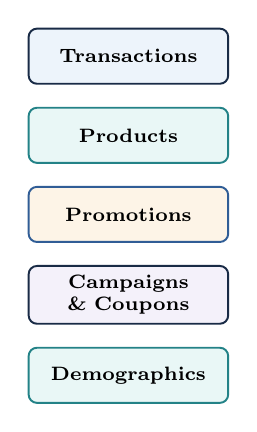
\begin{tikzpicture}[node distance=0.28cm]
\node (t) [flow] {\textbf{Transactions}};
\node (p) [flowteal, below=of t] {\textbf{Products}};
\node (pr) [floworange, below=of p] {\textbf{Promotions}};
\node (c) [flowpurple, below=of pr] {\textbf{Campaigns \\ \& Coupons}};
\node (d) [flowteal, below=of c] {\textbf{Demographics}};
\end{tikzpicture}
\end{center}
\end{column}
\end{columns}
\vfill
\begin{center}\scriptsize\color{MediumGray}Source: \href{https://www.dunnhumby.com/source-files/}{Dunnhumby -- The Complete Journey}\end{center}
\end{frame}

% =========================================================
% 6 DATA PARAMETERS
% =========================================================
\begin{frame}{Dataset: From Raw Data to OR Parameters}
\vspace{0.1cm}
\begin{center}\scriptsize\color{MediumGray}The raw tables will be transformed into the parameters required by the two optimization models.\end{center}
\vspace{0.2cm}
\begin{columns}[T]
\begin{column}{0.32\textwidth}
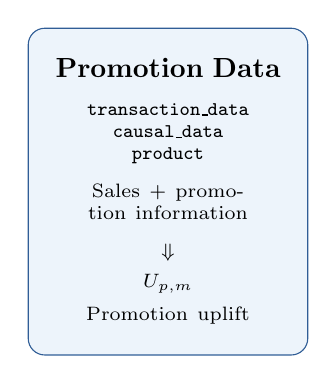
\begin{tikzpicture}
\node[rectangle,rounded corners=6pt,draw=Blue,fill=LightBlue,minimum width=3.55cm,minimum height=4.15cm,text width=3.15cm,align=center]{
\textbf{Promotion Data}\\[2mm]
\scriptsize\texttt{transaction\_data}\\
\scriptsize\texttt{causal\_data}\\
\scriptsize\texttt{product}\\[2mm]
Sales + promotion information\\[2mm]
$\Downarrow$\\[1mm]
\textbf{$U_{p,m}$}\\
Promotion uplift};
\end{tikzpicture}
\end{column}
\begin{column}{0.32\textwidth}
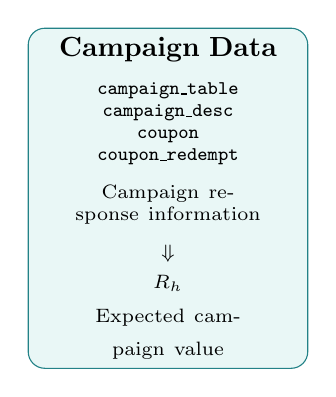
\begin{tikzpicture}
\node[rectangle,rounded corners=6pt,draw=Teal,fill=LightTeal,minimum width=3.55cm,minimum height=4.15cm,text width=3.15cm,align=center]{
\textbf{Campaign Data}\\[2mm]
\scriptsize\texttt{campaign\_table}\\
\scriptsize\texttt{campaign\_desc}\\
\scriptsize\texttt{coupon}\\
\scriptsize\texttt{coupon\_redempt}\\[2mm]
Campaign response information\\[2mm]
$\Downarrow$\\[1mm]
\textbf{$R_h$}\\
Expected campaign value};
\end{tikzpicture}
\end{column}
\begin{column}{0.32\textwidth}
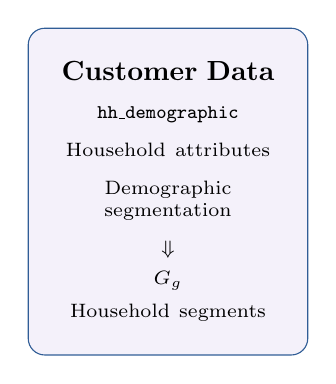
\begin{tikzpicture}
\node[rectangle,rounded corners=6pt,draw=Blue,fill=LightPurple,minimum width=3.55cm,minimum height=4.15cm,text width=3.15cm,align=center]{
\textbf{Customer Data}\\[2mm]
\scriptsize\texttt{hh\_demographic}\\[2mm]
Household attributes\\[2mm]
Demographic segmentation\\[2mm]
$\Downarrow$\\[1mm]
\textbf{$G_g$}\\
Household segments};
\end{tikzpicture}
\end{column}
\end{columns}
\vspace{0.25cm}
\begin{center}\textcolor{Navy}{\textbf{Raw Data $\rightarrow$ Historical Parameter Estimation $\rightarrow$ OR Models}}\end{center}
\end{frame}

% =========================================================
% 7 METHODOLOGY
% =========================================================
\begin{frame}{Proposed Methodology}
\vspace{0.02cm}
\begin{center}
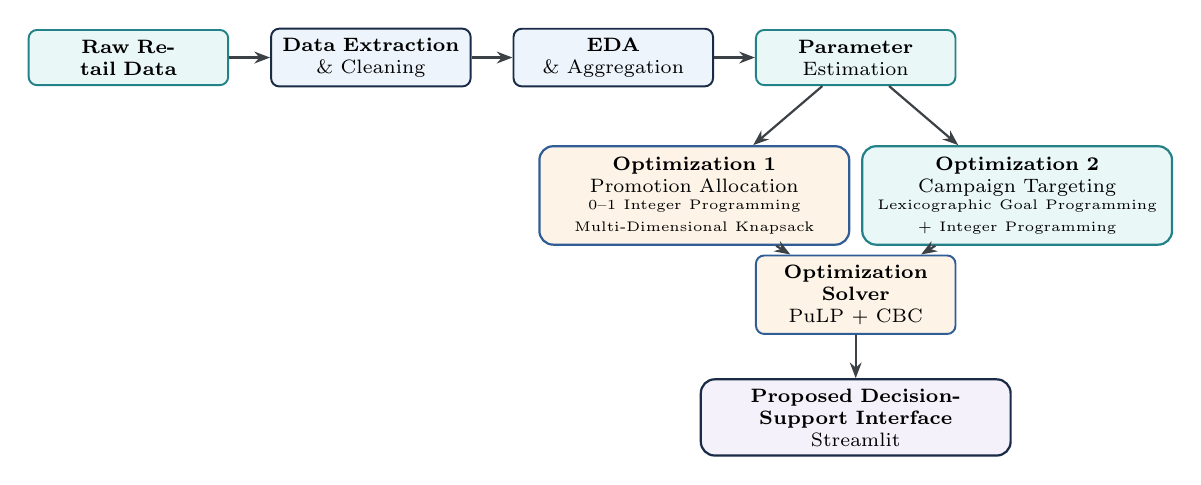
\begin{tikzpicture}[node distance=0.55cm and 0.52cm]
\node (raw) [flowteal] {\textbf{Raw Retail Data}};
\node (clean) [flow, right=of raw] {\textbf{Data Extraction}\\\& Cleaning};
\node (eda) [flow, right=of clean] {\textbf{EDA}\\\& Aggregation};
\node (param) [flowteal, right=of eda] {\textbf{Parameter}\\Estimation};
\draw[arr] (raw)--(clean); \draw[arr] (clean)--(eda); \draw[arr] (eda)--(param);

\node (promo) [model, below=0.75cm of param, xshift=-2.05cm] {\textbf{Optimization 1}\\Promotion Allocation\\\tiny 0--1 Integer Programming\\\tiny Multi-Dimensional Knapsack};
\node (camp) [modelteal, below=0.75cm of param, xshift=2.05cm] {\textbf{Optimization 2}\\Campaign Targeting\\\tiny Lexicographic Goal Programming\\\tiny + Integer Programming};
\draw[arr] (param)--(promo); \draw[arr] (param)--(camp);

\node (solver) [floworange, below=0.75cm of $(promo)!0.5!(camp)$] {\textbf{Optimization Solver}\\PuLP + CBC};
\draw[arr] (promo)--(solver); \draw[arr] (camp)--(solver);

\node (ui) [outputbox, below=0.55cm of solver] {\textbf{Proposed Decision-Support Interface}\\Streamlit};
\draw[arr] (solver)--(ui);
\end{tikzpicture}
\end{center}
\vspace{0.02cm}
\begin{center}\tiny\color{MediumGray}Historical data will provide the coefficients used by the optimization models.\end{center}
\end{frame}

% =========================================================
% 8 OPT 1
% =========================================================
\begin{frame}{Optimization 1: Promotion Allocation}
\vspace{0.05cm}
\begin{center}\color{Blue}\textbf{0--1 Integer Programming with Multi-Dimensional Knapsack Structure}\end{center}
\vspace{0.2cm}
\begin{columns}[T]
\begin{column}{0.31\textwidth}
\begin{block}{Decision Variable}
\centering
$ x_{p,m}\in\{0,1\} $
\vspace{1mm}
\raggedright
Select at most one promotion type for each product:
\[
m\in\{\text{Display, Mailer, Both}\}
\]
\end{block}
\end{column}
\begin{column}{0.35\textwidth}
\begin{block}{Objective}
\centering
\[
\boxed{\displaystyle
\max Z=\sum_p\sum_m U_{p,m}x_{p,m}}
\]
\vspace{-1mm}
\raggedright
Maximize estimated incremental sales.
\end{block}
\end{column}
\begin{column}{0.29\textwidth}
\begin{block}{Capacity Constraints}
\[
\sum_{p,m}x_{p,m}\le K
\]
\[
\sum_p x_{p,D}+\sum_p x_{p,B}\le D_{\max}
\]
\[
\sum_p x_{p,M}+\sum_p x_{p,B}\le M_{\max}
\]
\end{block}
\end{column}
\end{columns}
\vspace{0.35cm}
\begin{center}

\begin{tikzpicture}[node distance=0.75cm]
\node (a) [flow] {\textbf{Products}};
\node (b) [floworange, right=of a] {\textbf{Promotion Choice}\\Display / Mailer / Both};
\node (c) [flowteal, right=of b] {\textbf{Resource Constraints}};
\node (d) [flowpurple, right=of c] {\textbf{Maximum}\\Incremental Sales};
\draw[arr](a)--(b);\draw[arr](b)--(c);\draw[arr](c)--(d);
\end{tikzpicture}
\end{center}
\end{frame}

% =========================================================
% 9 OPT 2
% =========================================================
\begin{frame}{Optimization 2: Campaign Targeting}
\vspace{0.05cm}
\begin{center}\color{Teal}\textbf{Two-Stage Lexicographic Goal Programming + Integer Programming}\end{center}
\vspace{0.25cm}
\begin{columns}[T]
\begin{column}{0.46\textwidth}
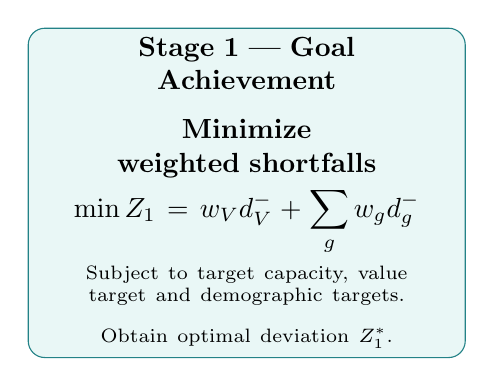
\begin{tikzpicture}
\node[rectangle,rounded corners=6pt,draw=Teal,fill=LightTeal,minimum width=5.55cm,minimum height=3.45cm,text width=5.05cm,align=center]{
\textbf{Stage 1 --- Goal Achievement}\\[2mm]
\textbf{Minimize weighted shortfalls}\\[1mm]
$\displaystyle \min Z_1=w_Vd_V^-+\sum_gw_gd_g^-$\\[1mm]
\scriptsize Subject to target capacity, value target and demographic targets.\\[1mm]
Obtain optimal deviation $Z_1^*$.
};
\end{tikzpicture}
\end{column}
\begin{column}{0.08\textwidth}
\vspace{1.5cm}\centering{\Large$\Longrightarrow$}
\end{column}
\begin{column}{0.46\textwidth}
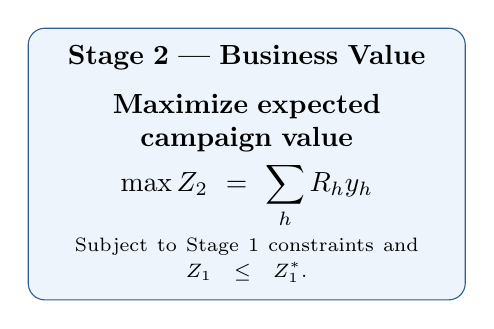
\begin{tikzpicture}
\node[rectangle,rounded corners=6pt,draw=Blue,fill=LightBlue,minimum width=5.55cm,minimum height=3.45cm,text width=5.05cm,align=center]{
\textbf{Stage 2 --- Business Value}\\[2mm]
\textbf{Maximize expected campaign value}\\[1mm]
$\displaystyle \max Z_2=\sum_hR_hy_h$\\[1mm]
\scriptsize Subject to Stage 1 constraints and\\[-1mm]
$Z_1\le Z_1^*$.
};
\end{tikzpicture}
\end{column}
\end{columns}
\vspace{0.25cm}
\begin{center}\textcolor{Navy}{\textbf{Strategic Goal Achievement $\rightarrow$ Business Value Maximization}}\end{center}
\end{frame}

% =========================================================
% 10 TOOLS
% =========================================================
\begin{frame}{Tools \& Technologies}
\vspace{0.25cm}
\begin{center}
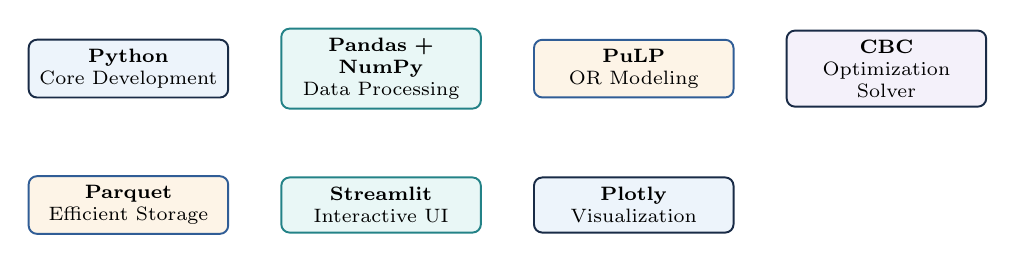
\begin{tikzpicture}[node distance=0.65cm]
\node (p) [flow] {\textbf{Python}\\Core Development};
\node (d) [flowteal, right=of p] {\textbf{Pandas + NumPy}\\Data Processing};
\node (l) [floworange, right=of d] {\textbf{PuLP}\\OR Modeling};
\node (c) [flowpurple, right=of l] {\textbf{CBC}\\Optimization Solver};
\node (s) [flowteal, below=0.85cm of d] {\textbf{Streamlit}\\Interactive UI};
\node (v) [flow, right=of s] {\textbf{Plotly}\\Visualization};
\node (q) [floworange, left=of s] {\textbf{Parquet}\\Efficient Storage};
\end{tikzpicture}
\end{center}
\vspace{0.55cm}
\begin{center}

\begin{tikzpicture}
\node[rectangle,rounded corners=5pt,draw=Navy,fill=LightGray,minimum width=10.5cm,minimum height=0.65cm,text width=10.5cm,align=center]{\textbf{Data Processing $\rightarrow$ OR Modeling $\rightarrow$ Optimization $\rightarrow$ Decision Support}};
\end{tikzpicture}
\end{center}
\vspace{0.35cm}
\begin{center}\scriptsize\color{MediumGray}The technology stack supports data preparation, mathematical modeling, optimization and the proposed interactive interface.\end{center}
\end{frame}

% =========================================================
% 11 SYSTEM
% =========================================================
\begin{frame}{Proposed Decision-Support Framework}
\vspace{0.05cm}
\begin{center}
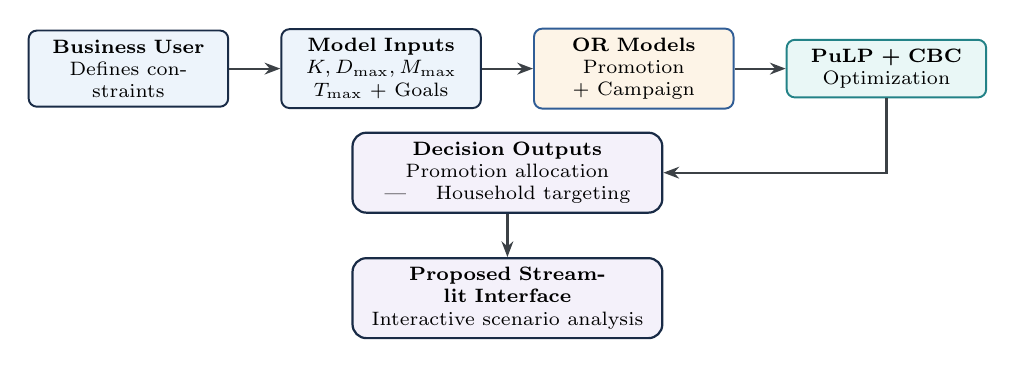
\begin{tikzpicture}[node distance=0.55cm and 0.65cm]
\node (u) [flow] {\textbf{Business User}\\Defines constraints};
\node (i) [flow, right=of u] {\textbf{Model Inputs}\\$K,D_{\max},M_{\max}$\\$T_{\max}$ + Goals};
\node (m) [floworange, right=of i] {\textbf{OR Models}\\Promotion + Campaign};
\node (s) [flowteal, right=of m] {\textbf{PuLP + CBC}\\Optimization};
\draw[arr](u)--(i);\draw[arr](i)--(m);\draw[arr](m)--(s);
\node (o) [outputbox, below=0.8cm of $(i)!0.5!(m)$] {\textbf{Decision Outputs}\\Promotion allocation \quad | \quad Household targeting};
\node (ui) [outputbox, below=0.55cm of o] {\textbf{Proposed Streamlit Interface}\\Interactive scenario analysis};
\draw[arr](s) |- (o);\draw[arr](o)--(ui);
\end{tikzpicture}
\end{center}
\vspace{0.1cm}
\begin{columns}[T]
\begin{column}{0.46\textwidth}
\begin{block}{User Controls}
\scriptsize
Promotion capacity; display and mailer limits; campaign targeting capacity; demographic goals.
\end{block}
\end{column}
\begin{column}{0.46\textwidth}
\begin{block}{Expected Outputs}
\scriptsize
Selected product promotions; selected households; expected business value; goal deviations.
\end{block}
\end{column}
\end{columns}
\end{frame}

% =========================================================
% 12. CONCLUSION
% =========================================================
\begin{frame}{Conclusion}

\vspace{0.35cm}

\begin{itemize}

    \item The proposed framework applies Operations Research to
    retail promotion allocation and campaign targeting.

    \vspace{0.35cm}

    \item Historical data from Dunnhumby -- The Complete Journey
    will be transformed into parameters for the optimization models.

    \vspace{0.35cm}

    \item Integer Programming and Lexicographic Goal Programming
    will address operational and strategic retail constraints.

    \vspace{0.35cm}

    \item The proposed decision-support system will enable
    data-driven retail planning through interactive scenario analysis.

\end{itemize}

\end{frame}

\end{document}
